\documentclass[11pt,a5paper]{article}
\usepackage{xcolor}
\usepackage[T1]{fontenc}
\usepackage[utf8]{inputenc}
\usepackage[italian]{babel}
\usepackage{alltt}
\usepackage{scrextend}
\usepackage{geometry}
\usepackage[default]{opensans}
\usepackage{eso-pic}
\usepackage{tikz}
\usepackage{titlesec}
\usepackage[most]{tcolorbox}
\definecolor{block-gray}{gray}{0.82}
\newtcolorbox{myquote}{colback=block-gray,grow to right by=-10mm,grow to left by=-10mm, boxrule=0pt,boxsep=0pt,breakable}

\usepackage{titlesec}
\usepackage{graphicx}
\usepackage{transparent}
\usepackage{ifthen}
\usepackage{changepage}
\usepackage{fdsymbol}
\usepackage[final,kerning=true,spacing=true,tracking=true,activate={true,nocompatibility},stretch=10,shrink=10]{microtype}

\SetTracking{encoding={*}, shape=sc}{0}
\SetExtraKerning[unit=space]{encoding=T1}{'={160,280},”={250,0},“={0,100}}

\newlength{\sectionnumlen}
\setlength{\sectionnumlen}{30pt}

\titleformat{\section}%
{\fontfamily{ppl}\selectfont\fontsize{16}{24}\selectfont\scshape\bfseries}%
{\makebox[\sectionnumlen][l]{\bfseries\scshape\thesection}}%
{0mm}%
{}%
[\vskip -0.1cm plus 0.1cm minus 0.1cm]%

% Per aggiungere il logo SNS in trasparenza ad alcune pagine
\newif\iflogo
\AddToShipoutPictureBG{
  \iflogo{%
    \put(280,390){%
      \transparent{0.17}
\includegraphics[width=3.5cm]{images/logo_SNS_nero}%
    }%
  }\else\fi%
}

\newcommand{\RIT}{%
  \vspace*{-0.3em}%
  {~\hfill{\fontfamily{ppl}\selectfont $\vardiamondsuit${\hskip 0.5em}RIT.{\hskip 0.5em}$\vardiamondsuit$}\hfill~}%
  \vspace*{-0.3em}%
}

\newcommand{\ARIT}{%
  {\fontfamily{ppl}\selectfont RIT.}%
}

\newcommand{\RITB}{%
  \vspace*{-0.3em}%
  {~\hfill{\fontfamily{ppl}\selectfont $\vardiamondsuit${\hskip 0.5em}RIT. (x2){\hskip 0.5em}$\vardiamondsuit$}\hfill~}%
  \vspace*{-0.3em}%
}

\newcommand{\ALLREP}[1]{%
	{\fontfamily{ppl}\selectfont {\hskip 0.5em}(Tutto x#1){\hskip 0.5em}}%
}

\makeatletter
\renewcommand{\@seccntformat}[1]{%
  \begingroup
  \@nameuse{additional@cntformat#1}%
  {\@nameuse{the#1}}%
  \endgroup
  \quad
}
\newcommand{\setformat}[2]{%
  \@namedef{additional@cntformat#1}{#2}%
}
\makeatother

% \setformat{section}{\LARGE}

\definecolor{ourgray}{HTML}{606060}
\newcommand{\santanna}{{\normalsize s}ant'{\normalsize a}nna}
\newcommand{\subtitle}[1]{\vspace*{-0.7em}%
  {\makebox[\sectionnumlen][l]{}\textcolor{ourgray}{\fontsize{11.5}{16}\selectfont\it #1}}}
\renewcommand{\title}[1]{%
  \begin{center}%
    {\fontfamily{pag}\selectfont\scshape\Huge{#1}}%
  \end{center}%
}

\newlength{\aritlen}
\settowidth{\aritlen}{\ARIT: }

\newcommand{\aritskip}{\makebox[\aritlen][l]{}}

\newenvironment{canzone}{%
  \begin{adjustwidth}{\sectionnumlen}{}%
  \begin{alltt}\normalfont%
  }{%
  \end{alltt}%
  \end{adjustwidth}%
}

\begin{document}
\logofalse
\newgeometry{top=0mm,bottom=0mm,left=0mm,right=0mm}
\fontsize{13}{16}\selectfont
\setlength{\parindent}{0cm}
\setlength{\parskip}{1.0em plus 0.4em minus 0.2em}
\linespread{1.25}
\pagestyle{empty}

%% -- PRIMA DI COPERTINA
\leavevmode
\put(50,70){
  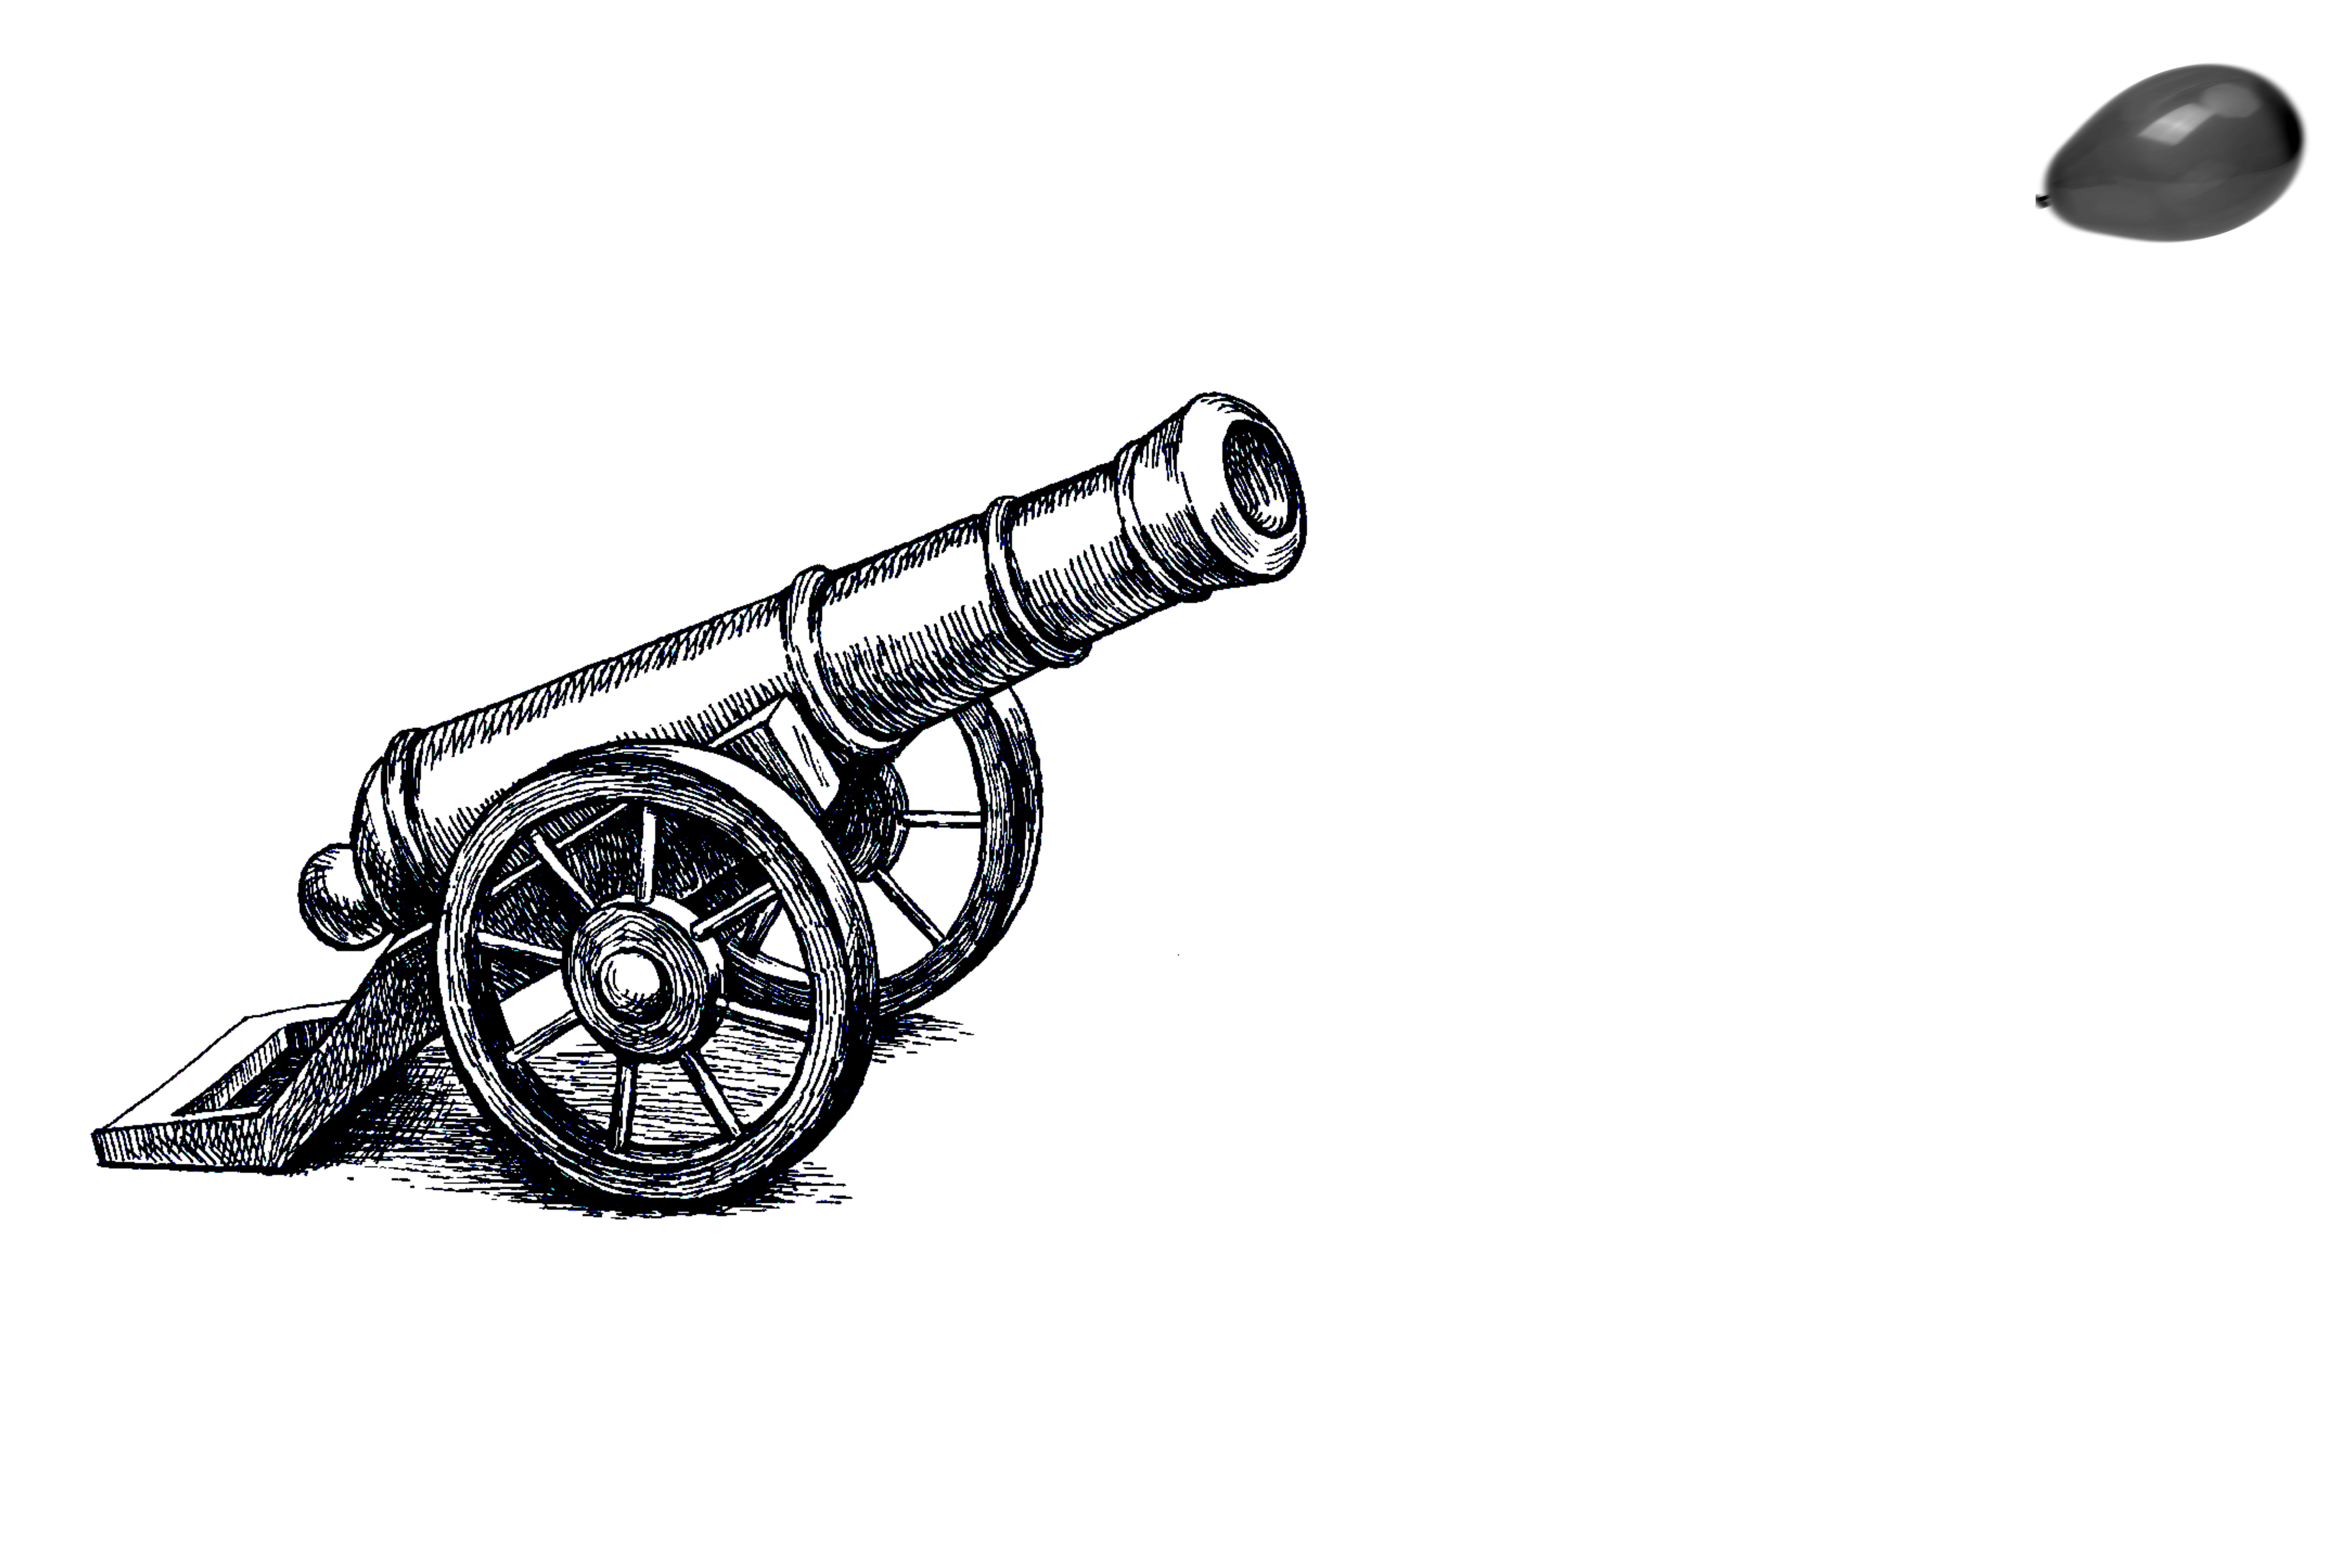
\includegraphics[width=0.70\textwidth]{images/miniatura}
}
\leavevmode
\put(-3,-1){
  
\includegraphics[width=\dimexpr\textwidth\relax,height=\dimexpr\textheight-0.05mm\relax]{images/cornice}
}
\leavevmode
\put(60,300){
  
\includegraphics[width=0.70\textwidth]{images/striscione}
}
\clearpage


\if twoside
\newgeometry{top=20mm,inner=20mm,outer=10mm,bottom=20mm}
\else
\newgeometry{top=20mm,left=15mm,right=15mm,bottom=20mm}
\fi
%% -- CITAZIONE E RINGRAZIAMENTI
\begin{myquote}\it
  Chi vince la guerra scrive la storia,\\
  chi perde la guerra scrive i giornali.
  
  {~\hfill\normalfont -- Gianni Cusumano}
\end{myquote}

\vfill

\begin{minipage}{0.80\textwidth}\fontsize{10}{15}\selectfont
  Cornice e Titolo di Marta Tasinato\\
  Adeguamento Immagini di Piero Lafiosca ed Enrico Polesel\\
  Correzione testi di Nicolò Campodonico\\
  Impaginazione e Layout di Dario Balboni
\end{minipage}
\clearpage


\logotrue
%% -- INIZIO DEL CANZONIERE
\title{Canzoniere di Guerra}
\title{della}
\title{Scuola Normale Superiore}
\begin{center}%
	{\fontfamily{pag}\selectfont\scshape\Large{(Versione CD)}}%
\end{center}%

\section{Alla Normale urrà!}
\subtitle{Sulla melodia di “When Johnny comes marching home”}
\begin{canzone}
È pronta la Normale per le avversità:
Abbiam giurato tutti non aver pietà!
I gavettoni alla fanteria,
Dalle finestre l’artiglieria,
Fremono gli idranti.
Per la Normale urrà!

Non hanno i santannini alcuna dignità:
Son tutti dei fascisti figli di papà;
Non hanno fatto neanche un bidet
Sin dal lontano sessantatré:
È arrivato il puzzo
Sino in Normale già!

Vedendoli fuggire ed implorar pietà,
Mostriamo ai loro anziani cos’è l’umiltà
E da sevizie ridicole
Salviam le loro matricole,
Che dovran la vita
Alla Normale, urrà!

E da sevizie ridicole
Salviam le loro matricole,
Che dovran la vita
Alla Normale, urrà!
(Alla Normale, urra!) (x2)
\end{canzone}

%\section{\santanna\ merda}
\begin{canzone}
Sant’Anna merda, Sant’Anna colera,
Sei la rovina dell’Italia intera.
O santannino, lavora duro
Che alla Normale devi dare pure il culo!
Santannino, figlio di puttana!
Santannino, figlio di puttana! 
(ad libitum)
\end{canzone}

\section{Scuola Normale trionferà}
\subtitle{Sulla melodia di “Bandiera Rossa”}

\subtitle{Tonalità possibilmente bassa}
\begin{canzone}
Puzza di fogna, ti attacca il tifo,
Pidocchi e rogna: fa proprio schifo!
È il santannino: è un animale,
Ma la Normale lo domerà.

Scuola Normale la trionferà,
Scuola Normale la trionferà,
E il santannino che la sfiderà
Lavato con Perlana si ritirerà!

Noi integriamo gli operatori,
Campi finiti, quadritensori;
Mentre al Sant’Anna - che gran buffoni - 
Solo addizioni sapete far!

Scuola Normale la trionferà,
Scuola Normale la trionferà,
E il santannino che la sfiderà
Lavato con Perlana si ritirerà.

I santannini sono ingegneri,
sono giuristi, son parrucchieri.
Ma quale genio? Ma che eccellenza?
La vera scienza si fa in Normal!

Scuola Normale la trionferà,
Scuola Normale la trionferà,
Scuola Normale la trionferà,
Se liberiam Barbieri chi vi salverà?
Se liberiam Barbieri chi ci salverà?
\end{canzone}

\section{Son perdenti, son sfigati}
\subtitle{Sul canto tipico dei marines}

\subtitle{Ogni verso si canta due volte}
\begin{canzone}
Son perdenti, son sfigati
I giuristi e gli avvocati!
Gli ingegneri, che buffoni:
Sbaglian pure le addizioni!

Destinato è il santannino
Solo a fare lo spazzino!
Canta in cor la nostra truppa:
S.S.S.U.Puppa!
\end{canzone}

\section{Nella notte più nera}
\subtitle{Sulla melodia di “Let's Go“ del Coro dell’Armata Rossa}
\begin{canzone}
Nella notte più nera
Non cerchiamo il sole, mio signor!
Ma solo uno scudo e uno stemma bianco e blu
Che ci porti ancor più su, 
Ancor più su,
Su, su!
Uniti contro il male,
Lottiam per la Normale:
Vittoria noi cerchiam e arriverà!

Noi di folgore non armati
I cieli squarceremo, sì!
Ché di gavettoni tempesta sorgerà
Che affondi il Sant’Anna giù, 
Ancor più giù, 
Giù, giù!
Nell’abisso più infame,
Più delle loro brame
Di aver la dignità
Della Normal!

Come fiera testuggine
L’oscuro mare fermerem
E quando la luce infine tornerà
L’onda azzurra crescerà,
L’abbatterà 
Là, là!
Là nelle loro tane
Di sevizie inumane.
La Storia canterà:
Normale urrà!
\end{canzone}

\section{Sono gli scemi del \santanna}
\subtitle{Ogni verso si canta due volte}
\begin{canzone}
Ovunque voi andiate,
Noi ci siamo.
La genta ci domanda:
“Ma chi sono?”
Sono gli scemi del Sant’Anna,
Tutti segati alla Normale,
Che per cercar di rimediare
Vanno a far finta di studiare. 
\end{canzone}

\section{Lo han segato alla Scuola Normal}
\subtitle{Sulla melodia di “Whiskey in the Jar”, versione dei Dubliners}
\begin{canzone}
Come un animale si sveglia ogni mattino,
Avviterà bulloni: è infelice il santannino.
Voleva esser fisico, studiare la natura,
Ma della sua ignoranza sì che c’è da aver paura!

\ARIT: L’han segato alla Scuola Normal
\aritskip Assieme ad altri segati,
\aritskip Assieme ad altri segati
\aritskip Lui è andato a star.

D’estate una mattina lui è andato all’ammissione:
Credeva d’esser genio, ma era solo un gran coglione;
Di fronte a quei problemi non sapeva cosa fare:
Almeno le addizioni eran cosa da imparare.

\RIT

Qualche giorno dopo in Santa Caterina
Gli chiedon se è capace ad avvitar la lampadina:
Lui prova a caso un verso, credendo sia lo stesso.
Al secondo tentativo finalmente viene ammesso.

\RIT

Da povera matricola, quand’era appena entrato,
Com’essere inferiore lui è stato seviziato.
Onora i suoi anziani, ritenendoli speciali:
Non sa d’esser finito dentro a un covo di animali.

\RIT

Solo tre anni dopo devon scriver le tesine:
Chiodi, viti oppure scienza delle merendine?
Anche da laureato lui continua a rosicare
Perché da un normalista avrebbe solo da imparare.

\RIT

Giunto al quinto anno la sua essenza ha rivelato:
Pelliccia attorno al corpo e cervello obnubilato.
Il suo pensiero fisso lo tormenta ogni ora:
Quella bocciatura, mamma mia se brucia ancora!

\RITB
\end{canzone}

%\section{Normale Olè}
\subtitle{Sulla melodia dell’inno della Sampdoria}
\begin{canzone}
Normale olè, Normale olè,
Forza Normale, Normale olè!
Normale olè, Normale olè,
Forza Normale, Normale olè!

Se le scuole sono tante,
La migliore resti tu:
Sei l'orgoglio del Priore
Che ci guida da lassù.
E la feccia santannina
Fu la nostra succursal,
Ora trema poverina,
Se ci sente cantar.

Normale olè, Normale olè,
Forza Normale, Normale olè!
Normale olè, Normale olè,
Forza Normale, ...Normale olè!
\end{canzone}

\section{Il ponte sul fiume Arno}
\begin{canzone}
Guarda, che cosa vedi là?
Sembra il culo d’un maial
e invece è un santannino
- steccò persino il test in Normal! -

Puzza come un animal.
Studia, ma resta un gran somar.
Merda di un santannino,
fatti vicino ti devo lavar!
\end{canzone}

%\section{Coro Napoletano per Maradona}
\begin{canzone}
O mama, mama, mama! O mama, mama, mama!
Sai perché mi batte il corazon? 
Ho ucciso un santannino, ho ucciso un santannino
Uè, mammà, l'ho tolto dai coglion!
\end{canzone}

\clearpage
\logofalse

INTERMEZZO
\clearpage


\logotrue
\section{Il santannino puzza}
\begin{canzone}
Il santannino puzza,
ma lo laveremo noi.
Se pure voi barate
non ci arrenderemo mai!
Con Vasco condottiero
e Beltram nostro dio,
nostro sarà il trionfo
e voi cadrete nell’oblio!
Nostro sarà il trionfo
e voi cadrete nell’oblio!

Il normalista è fiero,
non prova mai timor:
combatte per dar gloria
alla Normale Superior.
E abbiamo dalla nostra
anche la gravità...
Se un giorno mai scopriste
che anche l'acqua in basso va,
ma siete troppo scemi
e la Normale vincerà!
\end{canzone}

%\section{Noi vogliamo tanto bene}
\subtitle{Sulla base di “Noi vogliamo tanto bene alla Polizia Italiana”}
\begin{canzone}
Noi vogliamo tanto bene 
Al santannino boia,
Noi vogliamo tanto bene 
A quel gran figlio di troia!
\end{canzone}

%\section{Ma al \santanna\ no}
\begin{canzone}
Quasi tutta la gente ha un'igiene decente,
\textit{ma al \santanna no!}
Relazioni normali ci son tra gli animali,
\textit{ma al \santanna no!}
Moderarsi ai processi lo san fare anche i fessi,
\textit{ma al \santanna no!}
Quasi ovunque in natura si è trovata una cura,
\textit{ma al \santanna no!}

Disegnare una {\selectlanguage{greek}θ}eta lo fa un analfabeta,
\textit{ma al \santanna no!}
Cosa son le equazioni lo san pure i coglioni,
\textit{ma al \santanna no!}
Quattro conti azzeccati li fan pure i primati,
\textit{ma al \santanna no!}
L'intuizione geniale sempre abbonda in Normale,
\textit{ma al \santanna no!}

Urrà! Urrà! Urrà alla Normale!
Ma al \santanna no! \hspace{5em} {\small x4}
\begin{flushright} Scuola Superiore de che?
	Puppa! “Superiore” siam noi!
\end{flushright}Ma al \santanna... \hspace{1.5em} \textit{- segati -}
Ma al \santanna... no! \hspace{4em} {\small x2}

Dice il latinista qui nessuno è fascista,
\textit{ma al \santanna no!}
Ingegneri e avvocati, noi li abbiamo segati,
\textit{ma al \santanna no!}
E per questa rottura il gavettone è la cura,
\textit{ma al \santanna no!}
Noi ne abbiam centinaia, anzi, molte migliaia,
\textit{ma al \santanna no!}

Urrà! Urrà! Urrà alla Normale!
Ma al \santanna no! \hspace{5em} {\small x4}
\begin{flushright} Scuola Superiore de che?
Puppa! “Superiore” siam noi!
\end{flushright}Ma al \santanna... \hspace{1.5em} \textit{- segati -}
Ma al \santanna... no! \hspace{4em} {\small x2}
\end{canzone}

\section{Il sogno alla Normale}
\subtitle{Sulla melodia di “Il sogno di un Pisano”}
\begin{canzone}
Il sogno alla Normale è 
Svegliarsi la mattina
E veder bruciare 
Piazza Santa Caterina!

\ALLREP{3}
\end{canzone}

%\section{Benvenuti}
\subtitle{Sulla melodia di “La società dei Magnaccioni” di Lando Fiorini}
\begin{canzone}
E benvenuti ai santannini,
Ignoranti e anche cretini!
C’offrite l’ano,
E noi che famo?
C’avemo l’acqua e ve la tiriamo!
\end{canzone}

%\section{San Francesco}
\subtitle{Sulla melodia di “Stalingrado” degli Stormy Six}
\begin{canzone}
Fame e macerie dentro al Terzani:
Come il piombo combatte la Normal.
Strade di San francesco, 
Di acqua siete lastricate;
Combatte il nostro juggernaut 
Su mille barricate.

Sulla sua strada bagnata
Sant’Anna umiliata lo sa:
D’ora in poi troverà
La Normale che la laverà!

Generale da gonfiare gavettoni sin alle tre,
L’officina sforna scudi senza sosta:
Ma dentro al Carducci l’aria brucia come se
Non il solo onor fosse la posta.

Vinta la guerra noi a festeggiar,
Cento bicchieri per Fabio Martin.
E il santannino torna a casa,
Si lecca le ferite;
Vola uno scudo, un prode canta,
Il Priore ci sorride.

Sulla sua strada bagnata
Sant’Anna umiliata lo sa:
D’ora in poi troverà
La Normale che la laverà!
\end{canzone}

%\section{Siam Venuti fin qua}
\begin{canzone}
Siam venuti fin qua, siam venuti fin qua
Per vedere il Sant'Anna affogar!
\end{canzone}

\section{Sit triumphans, o Schola Normalis}
\subtitle{Sulla melodia di “Salve invicta Juditha formosa” di A. Vivaldi}

\subtitle{Si ripete tutto due volte a gruppi di due versi, tranne i vivat}
\begin{canzone}
Sis triumphans, o Schola Normalis,
Mundi splendor, spes nostrae salutis,\hfill (salutis)
Summae norma tu vere virtutis,
Linguae, artis et scientiae studi\underline{o}sa!

Sanctae Annae sic bestia domata
Triumphatrix sit scientiae regina,\hfill (regina)
Et placata sua ira divina,
Normalista nunc studet in p\underline{a}ce.

Vivat, vivat, vivat Normalis!
Vivat, vivat, vivat Normalis!
\end{canzone}

%\section{Settimo Comandamento}
\begin{canzone}
Santannino, brutto coglione,
Potevi rubare al Test d'Ammissione!
(ad libitum)
\end{canzone}

%\section{Che confusione}
\subtitle{Basata su “Sarà perché ti amo” dei Ricchi e Poveri}
\begin{canzone}
Che confusione!
Sarà perché offendiamo
Uno studente
Che non sa l’italiano,
Balbuziente
E non si capisce niente:
Il santannino
È proprio un deficiente!
\end{canzone}

%\section{Poveri Pirla}
\begin{canzone}
Poveri pirla,
Scuola derisa
Ma voi credete di essere capi di Pisa!

Sempre muti,
Cariche zero,
Più che una scuola sembrate un cimitero!

Sant'Anna merda! (ad libitum)
\end{canzone}

%\section{Youporn}
\subtitle{Sul ritornello di “Carneval de Paris” di Wender e Paolo Noise}
\begin{canzone}
Youporn, Youporn, Youporn!
Le Santannine le troviamo
a novanta su Youporn!
\end{canzone}

%\section{Ribadiamo un po' il concetto}
\subtitle{Usualmente cantato dopo “Youporn”}
\begin{canzone}
Ribadiamo un po' il concetto:
Cagne, cagne, cagne, cagne!
Cagne, cagne, cagne, cagne!
\end{canzone}

\section{Priore ciao}
\begin{canzone}
Una mattina mi son svegliato
- o priore ciao, priore ciao, priore ciao, ciao, ciao! -
Una mattina mi son svegliato
e ho trovato il santannin.

O Normalista, portami via
- o priore ciao, priore ciao, priore ciao, ciao, ciao! -
O Normalista, portami via,
questo puzza da morir.

E se io muoio con il mio scudo
- o priore ciao, priore ciao, priore ciao, ciao, ciao! -
E se io muoio con il mio scudo,
tu mi devi seppellir.

E seppellire là in Carovana
- o priore ciao, priore ciao, priore ciao, ciao, ciao! -
E seppellire là in Carovana
sotto l'ombra di Beltram.

\clearpage
Tutti i Pisani che passeranno
- o priore ciao, priore ciao, priore ciao, ciao, ciao! -
Tutti i Pisani che passeranno
mi offriranno un gavetton.

Questa è la bomba del Normalista
- o priore ciao, priore ciao, priore ciao, ciao, ciao! -
Questa è la bomba del Normalista
morto con lo scudo in man.

Questa è la bomba del Normalista
morto con lo scudo in man!
\end{canzone}

%\section{Il \santanna\ è}

\subtitle{Dal ritornello di “L'amico è”}
\begin{canzone}
Eh il Sant'Anna è
La scuola più infame che c’è.
Quando indossa la divisa un leone è,
Ma nella vita sai che gente c’è
Di merda!
\end{canzone}

%\section{L'importante è Partecipare!}
\begin{canzone}
Santannino non ti incazzare
L'importante è partecipare!
\end{canzone}

\section{L'Arno mormorava}
{\setstretch{1.2}\fontsize{13}{16}\selectfont
\begin{canzone}
L'Arno mormorava
calmo e placido di fronte
ai primi allievi in marcia sopra il ponte.
L'esercito avanzava,
trasportava i propri scudi,
mostrando al vento i fieri petti ignudi.

Carrelli ovunque pien di gavettoni!
Andavano a lavar quei gran puzzoni!

S'udiva intanto dalle vie d'intorno
il forte canto ed il suonar del corno.
Era il gran grido delle invitte schiere.

E l'Arno mormorò:
"Non passa l'ingegnere!"

Ma dopo la battaglia
si parlò di codardia,
ch'era il nemico presto corso via.
Saliva la marmaglia
sulle scale in Cavalieri,
dava una foto in pasto a dei ciarlieri.

Giornali scrive certo non la storia
il santannino che grida vittoria.

Veniva intanto in mente a ogni buffone
il tempo dell'esame d'ammissione.
Credeva d'esser genio di sapere.

Ma il test comandò:
"Segato è l'ingegnere!"

E ritornò una sera
in San Francesco la tenzone:
si miser tutti quanti in formazione.
S'ergeva tra la schiera
maestoso un gran fortino:
sottrasse ogni speranza al santannino!

Carrelli, ultrà e scudi ancor più grossi
e il fuoco e i calici scottanti e rossi!

Cercò la feccia allor di rimediare
Le scale in Carovana di occupare
Ma i Normalisti eran lì a tenere.

La piazza comandò:
"Indietro va', ingegnere!"

E indietreggiò sconfitto
fino in Santa Caterina,
si chiuse nella sua volgar latrina.
Placatosi il conflitto
tra le schiere il Costruttore
apparve assieme al nostro Gran Priore!

Sancì allora questa sacra vista
la nobile vittoria normalista!

Sicura casa e libere le scale
e tacque l'Arno e si zittì il giornale.
Sul patrio suolo vinti gl'ingegneri,

la scienza non trovò
spazzini e parrucchieri!
\end{canzone}
}

\section{Il vero Normalista}
\subtitle{Sulla melodia di “Katyusha“}
\begin{canzone}
Rischia il freddo il vero Normalista
Cinque esami, eppur bisogna andar
A conquistar piazza Santa Caterina
Dove sorge il covo santannin
A conquistar piazza Santa Caterina
Dove sorge il covo santannin

Ogni collegio è pieno di fervore
Ogni soldato brama di lavar
Nella notte lo guida il Gran Priore
Forte il cuore e il braccio nel lanciar
Nella notte lo guida il Gran Priore
Forte il cuore e il braccio nel lanciar

Se ci coglie in testa un gavettone
Dura vendetta sarà della Normal
Ormai sicura è la sorte del buffone
santannino vile traditor
Ormai sicura è la sorte del buffone
santannino vile traditor

Cessa il fuoco, lo scudo si riposa
Torna a casa fiera la Normal
Celebrando l'armata più gloriosa
Vittoriosi, alfin asciutti siam
Celebrando l'armata più gloriosa
Vittoriosi, alfin asciutti siam
Celebrando l'armata più gloriosa
Vittoriosi, alfin asciutti siam
\end{canzone}

\clearpage
\logofalse
\newgeometry{top=0mm,bottom=0mm,left=0mm,right=0mm}
%% -- ULTIMA DI COPERTINA
\leavevmode
\put(55,125){
  {\transparent{0.8}
\includegraphics[width=0.70\textwidth]{images/fregio}}
}
\leavevmode
\put(-4,0){
  
\includegraphics[width=\dimexpr\textwidth\relax,height=\dimexpr\textheight-0.1mm\relax]{images/cornice}
}


\end{document}

